\documentclass{article}
% Layout replica of the NeurIPS style. For submission: replace with \usepackage{neurips_2026} (official file).
\usepackage{neurips_replica}
\usepackage{amsmath,amssymb,amsthm,bm}
\usepackage{graphicx,booktabs,xcolor,array,multirow}
\usepackage[numbers,sort&compress]{natbib}
\usepackage[colorlinks=true,linkcolor=blue!55!black,citecolor=blue!55!black,urlcolor=blue!55!black]{hyperref}
\usepackage[capitalize,noabbrev]{cleveref}
\usepackage{enumitem,needspace}
\usepackage{tikz}
\usetikzlibrary{positioning,arrows.meta,fit,backgrounds,calc,shapes.geometric}
\setlist{itemsep=1pt,topsep=2pt,leftmargin=1.4em}
\newcolumntype{L}[1]{>{\raggedright\arraybackslash}p{#1}}
\newtheorem{proposition}{Proposition}
\theoremstyle{definition}\newtheorem{definition}{Definition}
\newcommand{\errClVal}{0.127\,$\pm$\,0.004}
\newcommand{\errClValMean}{0.127}
\newcommand{\mseClVal}{0.73\,$\pm$\,0.07}
\newcommand{\mseClValMean}{0.73}
\newcommand{\errClDec}{0.125\,$\pm$\,0.003}
\newcommand{\errClDecMean}{0.125}
\newcommand{\mseClDec}{0.73\,$\pm$\,0.10}
\newcommand{\mseClDecMean}{0.73}
\newcommand{\errClOodG}{0.429\,$\pm$\,0.014}
\newcommand{\errClOodGMean}{0.429}
\newcommand{\mseClOodG}{2.06\,$\pm$\,0.06}
\newcommand{\mseClOodGMean}{2.06}
\newcommand{\errClOodD}{0.147\,$\pm$\,0.003}
\newcommand{\errClOodDMean}{0.147}
\newcommand{\mseClOodD}{0.78\,$\pm$\,0.08}
\newcommand{\mseClOodDMean}{0.78}
\newcommand{\rtwoClsinthetaVal}{0.98\,$\pm$\,0.01}
\newcommand{\rtwoClsinthetaValMean}{0.98}
\newcommand{\rtwoClsinthetaDec}{0.98\,$\pm$\,0.01}
\newcommand{\rtwoClsinthetaDecMean}{0.98}
\newcommand{\rtwoClcosthetaVal}{0.98\,$\pm$\,0.01}
\newcommand{\rtwoClcosthetaValMean}{0.98}
\newcommand{\rtwoClcosthetaDec}{0.98\,$\pm$\,0.01}
\newcommand{\rtwoClcosthetaDecMean}{0.98}
\newcommand{\rtwoClomegaVal}{0.98\,$\pm$\,0.01}
\newcommand{\rtwoClomegaValMean}{0.98}
\newcommand{\rtwoClomegaDec}{0.98\,$\pm$\,0.01}
\newcommand{\rtwoClomegaDecMean}{0.98}
\newcommand{\rtwoClgravityVal}{0.02\,$\pm$\,0.01}
\newcommand{\rtwoClgravityValMean}{0.02}
\newcommand{\rtwoClgravityDec}{0.02\,$\pm$\,0.01}
\newcommand{\rtwoClgravityDecMean}{0.02}
\newcommand{\rtwoCldampingVal}{-0.01\,$\pm$\,0.02}
\newcommand{\rtwoCldampingValMean}{-0.01}
\newcommand{\rtwoCldampingDec}{-0.02\,$\pm$\,0.01}
\newcommand{\rtwoCldampingDecMean}{-0.02}
\newcommand{\rtwoClrednessVal}{0.60\,$\pm$\,0.53}
\newcommand{\rtwoClrednessValMean}{0.60}
\newcommand{\rtwoClrednessDec}{0.60\,$\pm$\,0.53}
\newcommand{\rtwoClrednessDecMean}{0.60}
\newcommand{\intShiftCl}{0.013\,$\pm$\,0.006}
\newcommand{\intShiftClMean}{0.013}
\newcommand{\intGimpCl}{-0.25\,$\pm$\,0.53}
\newcommand{\intGimpClMean}{-0.25}
\newcommand{\intGprobeCl}{0.02\,$\pm$\,0.16}
\newcommand{\intGprobeClMean}{0.02}
\newcommand{\cosGRCl}{0.04\,$\pm$\,0.15}
\newcommand{\cosGRClMean}{0.04}
\newcommand{\steerCCl}{0.007\,$\pm$\,0.005}
\newcommand{\steerCClMean}{0.007}
\newcommand{\steerRCl}{0.014\,$\pm$\,0.013}
\newcommand{\steerRClMean}{0.014}
\newcommand{\aucClGKnn}{0.58\,$\pm$\,0.02}
\newcommand{\aucClGKnnMean}{0.58}
\newcommand{\aucClGMaha}{0.58\,$\pm$\,0.02}
\newcommand{\aucClGMahaMean}{0.58}
\newcommand{\aucClGPrange}{0.50\,$\pm$\,0.00}
\newcommand{\aucClGPrangeMean}{0.50}
\newcommand{\aucClGKin}{0.54\,$\pm$\,0.06}
\newcommand{\aucClGKinMean}{0.54}
\newcommand{\aucClGLag}{0.66\,$\pm$\,0.04}
\newcommand{\aucClGLagMean}{0.66}
\newcommand{\aucClDKnn}{0.46\,$\pm$\,0.01}
\newcommand{\aucClDKnnMean}{0.46}
\newcommand{\aucClDMaha}{0.43\,$\pm$\,0.01}
\newcommand{\aucClDMahaMean}{0.43}
\newcommand{\aucClDPrange}{0.50\,$\pm$\,0.00}
\newcommand{\aucClDPrangeMean}{0.50}
\newcommand{\aucClDKin}{0.46\,$\pm$\,0.02}
\newcommand{\aucClDKinMean}{0.46}
\newcommand{\aucClDLag}{0.47\,$\pm$\,0.02}
\newcommand{\aucClDLagMean}{0.47}
\newcommand{\aucClDecKnn}{0.50\,$\pm$\,0.02}
\newcommand{\aucClDecKnnMean}{0.50}
\newcommand{\aucClDecMaha}{0.50\,$\pm$\,0.02}
\newcommand{\aucClDecMahaMean}{0.50}
\newcommand{\aucClDecPrange}{0.50\,$\pm$\,0.00}
\newcommand{\aucClDecPrangeMean}{0.50}
\newcommand{\aucClDecKin}{0.50\,$\pm$\,0.02}
\newcommand{\aucClDecKinMean}{0.50}
\newcommand{\aucClDecLag}{0.50\,$\pm$\,0.02}
\newcommand{\aucClDecLagMean}{0.50}
\newcommand{\errCoVal}{0.024\,$\pm$\,0.003}
\newcommand{\errCoValMean}{0.024}
\newcommand{\mseCoVal}{0.21\,$\pm$\,0.09}
\newcommand{\mseCoValMean}{0.21}
\newcommand{\errCoDec}{0.169\,$\pm$\,0.005}
\newcommand{\errCoDecMean}{0.169}
\newcommand{\mseCoDec}{0.92\,$\pm$\,0.07}
\newcommand{\mseCoDecMean}{0.92}
\newcommand{\errCoOodG}{0.431\,$\pm$\,0.014}
\newcommand{\errCoOodGMean}{0.431}
\newcommand{\mseCoOodG}{2.19\,$\pm$\,0.08}
\newcommand{\mseCoOodGMean}{2.19}
\newcommand{\errCoOodD}{0.175\,$\pm$\,0.008}
\newcommand{\errCoOodDMean}{0.175}
\newcommand{\mseCoOodD}{0.94\,$\pm$\,0.11}
\newcommand{\mseCoOodDMean}{0.94}
\newcommand{\rtwoCosinthetaVal}{0.97\,$\pm$\,0.01}
\newcommand{\rtwoCosinthetaValMean}{0.97}
\newcommand{\rtwoCosinthetaDec}{0.97\,$\pm$\,0.01}
\newcommand{\rtwoCosinthetaDecMean}{0.97}
\newcommand{\rtwoCocosthetaVal}{0.97\,$\pm$\,0.01}
\newcommand{\rtwoCocosthetaValMean}{0.97}
\newcommand{\rtwoCocosthetaDec}{0.96\,$\pm$\,0.01}
\newcommand{\rtwoCocosthetaDecMean}{0.96}
\newcommand{\rtwoCoomegaVal}{0.98\,$\pm$\,0.01}
\newcommand{\rtwoCoomegaValMean}{0.98}
\newcommand{\rtwoCoomegaDec}{0.98\,$\pm$\,0.01}
\newcommand{\rtwoCoomegaDecMean}{0.98}
\newcommand{\rtwoCogravityVal}{0.98\,$\pm$\,0.01}
\newcommand{\rtwoCogravityValMean}{0.98}
\newcommand{\rtwoCogravityDec}{-0.92\,$\pm$\,0.11}
\newcommand{\rtwoCogravityDecMean}{-0.92}
\newcommand{\rtwoCodampingVal}{-0.01\,$\pm$\,0.01}
\newcommand{\rtwoCodampingValMean}{-0.01}
\newcommand{\rtwoCodampingDec}{-0.01\,$\pm$\,0.01}
\newcommand{\rtwoCodampingDecMean}{-0.01}
\newcommand{\rtwoCorednessVal}{0.99\,$\pm$\,0.01}
\newcommand{\rtwoCorednessValMean}{0.99}
\newcommand{\rtwoCorednessDec}{0.98\,$\pm$\,0.01}
\newcommand{\rtwoCorednessDecMean}{0.98}
\newcommand{\intShiftCo}{0.251\,$\pm$\,0.007}
\newcommand{\intShiftCoMean}{0.251}
\newcommand{\intGimpCo}{7.97\,$\pm$\,1.13}
\newcommand{\intGimpCoMean}{7.97}
\newcommand{\intGprobeCo}{7.78\,$\pm$\,0.11}
\newcommand{\intGprobeCoMean}{7.78}
\newcommand{\cosGRCo}{1.00\,$\pm$\,0.00}
\newcommand{\cosGRCoMean}{1.00}
\newcommand{\steerCCo}{0.009\,$\pm$\,0.006}
\newcommand{\steerCCoMean}{0.009}
\newcommand{\steerRCo}{0.017\,$\pm$\,0.007}
\newcommand{\steerRCoMean}{0.017}
\newcommand{\aucCoGKnn}{0.57\,$\pm$\,0.01}
\newcommand{\aucCoGKnnMean}{0.57}
\newcommand{\aucCoGMaha}{0.57\,$\pm$\,0.01}
\newcommand{\aucCoGMahaMean}{0.57}
\newcommand{\aucCoGPrange}{0.50\,$\pm$\,0.00}
\newcommand{\aucCoGPrangeMean}{0.50}
\newcommand{\aucCoGKin}{0.54\,$\pm$\,0.05}
\newcommand{\aucCoGKinMean}{0.54}
\newcommand{\aucCoGLag}{0.69\,$\pm$\,0.04}
\newcommand{\aucCoGLagMean}{0.69}
\newcommand{\aucCoDKnn}{0.48\,$\pm$\,0.01}
\newcommand{\aucCoDKnnMean}{0.48}
\newcommand{\aucCoDMaha}{0.43\,$\pm$\,0.02}
\newcommand{\aucCoDMahaMean}{0.43}
\newcommand{\aucCoDPrange}{0.50\,$\pm$\,0.01}
\newcommand{\aucCoDPrangeMean}{0.50}
\newcommand{\aucCoDKin}{0.49\,$\pm$\,0.03}
\newcommand{\aucCoDKinMean}{0.49}
\newcommand{\aucCoDLag}{0.51\,$\pm$\,0.02}
\newcommand{\aucCoDLagMean}{0.51}
\newcommand{\aucCoDecKnn}{0.51\,$\pm$\,0.02}
\newcommand{\aucCoDecKnnMean}{0.51}
\newcommand{\aucCoDecMaha}{0.50\,$\pm$\,0.02}
\newcommand{\aucCoDecMahaMean}{0.50}
\newcommand{\aucCoDecPrange}{0.50\,$\pm$\,0.00}
\newcommand{\aucCoDecPrangeMean}{0.50}
\newcommand{\aucCoDecKin}{0.50\,$\pm$\,0.01}
\newcommand{\aucCoDecKinMean}{0.50}
\newcommand{\aucCoDecLag}{0.53\,$\pm$\,0.02}
\newcommand{\aucCoDecLagMean}{0.53}
\newcommand{\ratioDecVal}{7.1}
\newcommand{\ratioValClCo}{5.3}
\newcommand{\ratioIntCoCl}{19}
\newcommand{\nSeeds}{5}
\newcommand{\nTrainWin}{5000}
\newcommand{\nEpochs}{15}
\newcommand{\valPicksShortcut}{5}
\newcommand{\triArgClVal}{0.132\,$\pm$\,0.003}
\newcommand{\triArgClValMean}{0.132}
\newcommand{\triArgCoVal}{0.033\,$\pm$\,0.002}
\newcommand{\triArgCoValMean}{0.033}
\newcommand{\triArgCoDec}{0.171\,$\pm$\,0.005}
\newcommand{\triArgCoDecMean}{0.171}
\newcommand{\oraMeanG}{0.114\,$\pm$\,0.004}
\newcommand{\oraMeanGMean}{0.114}
\newcommand{\oraColG}{0.151\,$\pm$\,0.005}
\newcommand{\oraColGMean}{0.151}
\newcommand{\oraTrueG}{0.000\,$\pm$\,0.000}
\newcommand{\oraTrueGMean}{0.000}
\newcommand{\oraModelCl}{0.128\,$\pm$\,0.004}
\newcommand{\oraModelClMean}{0.128}
\newcommand{\oraModelCo}{0.169\,$\pm$\,0.005}
\newcommand{\oraModelCoMean}{0.169}
\newcommand{\idMlp}{0.01\,$\pm$\,0.02}
\newcommand{\idMlpMean}{0.01}
\newcommand{\idKnn}{-0.03\,$\pm$\,0.02}
\newcommand{\idKnnMean}{-0.03}
\newcommand{\idExact}{1.000\,$\pm$\,0.000}
\newcommand{\idExactMean}{1.000}
\newcommand{\idPixel}{-0.09\,$\pm$\,0.07}
\newcommand{\idPixelMean}{-0.09}
\newcommand{\readErrMean}{1.75\,$\pm$\,0.05}
\newcommand{\readErrMeanMean}{1.75}
\newcommand{\readErrMax}{5.2\,$\pm$\,0.0}
\newcommand{\readErrMaxMean}{5.2}
\newcommand{\doseACo}{0.025\,$\pm$\,0.001}
\newcommand{\doseACoMean}{0.025}
\newcommand{\doseACl}{0.002\,$\pm$\,0.001}
\newcommand{\doseAClMean}{0.002}
\newcommand{\doseBCo}{0.050\,$\pm$\,0.001}
\newcommand{\doseBCoMean}{0.050}
\newcommand{\doseBCl}{0.003\,$\pm$\,0.002}
\newcommand{\doseBClMean}{0.003}
\newcommand{\doseCCo}{0.097\,$\pm$\,0.003}
\newcommand{\doseCCoMean}{0.097}
\newcommand{\doseCCl}{0.007\,$\pm$\,0.004}
\newcommand{\doseCClMean}{0.007}
\newcommand{\doseDCo}{0.137\,$\pm$\,0.005}
\newcommand{\doseDCoMean}{0.137}
\newcommand{\doseDCl}{0.010\,$\pm$\,0.006}
\newcommand{\doseDClMean}{0.010}

\newcommand{\E}{\mathbb{E}}
\definecolor{cblue}{HTML}{2f5d8c}\definecolor{cred}{HTML}{b5443b}\definecolor{cgrey}{HTML}{6b6b6b}
\crefname{proposition}{Proposition}{Propositions}

\title{Why Physical AI Must Be Interpretable}
\author{Bhavith Chandra Challagundla\\
\normalfont Elemental Research Group \quad New York University\\
\normalfont\texttt{bc4066@nyu.edu}}

\begin{document}
\maketitle

\begin{abstract}
Physical AI systems increasingly act by consulting a learned world model: they imagine the consequences of candidate actions and execute the one whose imagined outcome is best. We argue that such systems cannot be certified by measuring their behavior, and that interpretability (evidence about which variables a world model represents and what those variables cause) is a technical requirement of physical AI. We support this with three results. (i) Accuracy on the training distribution does not identify the mechanism a world model has learned: a model that infers physics from a spurious cue can be exactly as accurate as one that has learned the physics, and only interventions separate them. (ii) A planner that optimizes against a world model selects that model's errors. The gap between predicted and realized outcomes therefore grows with the number of options compared, which makes held-out accuracy an optimistic estimate of decision quality. (iii) Physical failures are rare and irreversible, which puts behavioral certification out of statistical reach. In controlled experiments with pixel-based world models (5 seeds; all claims checked automatically), a model that learned a color shortcut for gravity is \ratioValClCo$\times$ \emph{more} accurate on validation data than a model trained on causal data, so validation selects it in every seed. Its error grows \ratioDecVal$\times$ once the shortcut breaks, and probes and interventions expose it using training data alone. When the models are used for planning, the realized cost at $N{=}\plNmax$ candidates is \plRatio$\times$ the predicted cost. We also report where simple interpretability tools fail, and we propose a program for building physical world models whose internal variables can be read, tested and trusted.
\end{abstract}

%=====================================================================
\section{Introduction}
%=====================================================================
\begin{figure}[t]
\centering
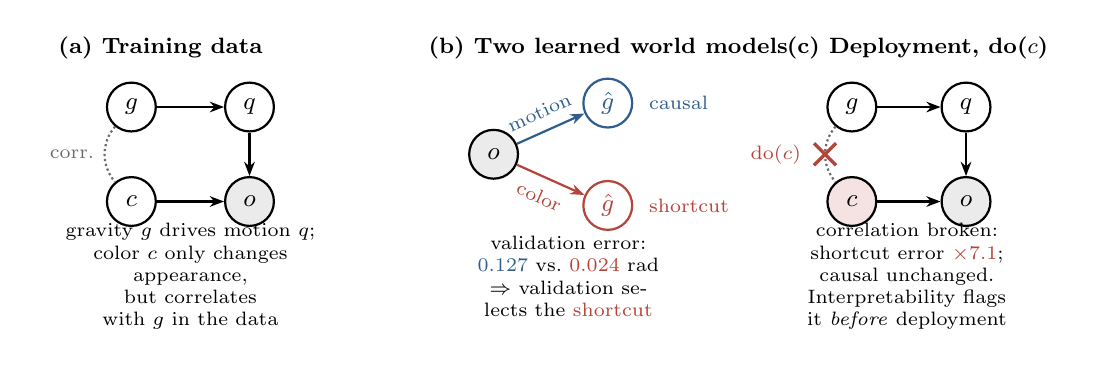
\begin{tikzpicture}[
  v/.style={circle, draw, thick, minimum size=0.62cm, inner sep=0pt, font=\small},
  obs/.style={v, fill=black!8},
  hid/.style={v, dashed},
  ar/.style={-{Stealth[length=1.8mm]}, thick},
  arb/.style={ar, cblue}, arr/.style={ar, cred},
  pt/.style={font=\footnotesize\bfseries, anchor=west},
  note/.style={font=\scriptsize, align=center, text width=3.9cm}]
% ---------- panel (a): data-generating process during training
\begin{scope}
\node[pt] at (-1.05,1.55) {(a) Training data};
\node[v] (g) at (0,0.8) {$g$};
\node[v] (c) at (0,-0.4) {$c$};
\node[v] (q) at (1.5,0.8) {$q$};
\node[obs] (o) at (1.5,-0.4) {$o$};
\draw[ar] (g) -- (q); \draw[ar] (q) -- (o); \draw[ar] (c) -- (o);
\draw[thick, densely dotted, cgrey] (g) to[bend right=40] node[left, font=\scriptsize, text=cgrey]{corr.} (c);
\node[note] at (0.75,-1.35) {gravity $g$ drives motion $q$;\\ color $c$ only changes appearance,\\ but correlates with $g$ in the data};
\end{scope}
% ---------- panel (b): two learned routes, identical validation error
\begin{scope}[xshift=4.6cm]
\node[pt] at (-0.95,1.55) {(b) Two learned world models};
\node[obs] (o2) at (0,0.2) {$o$};
\node[v, draw=cblue, text=cblue] (m) at (1.45,0.85) {$\hat g$};
\node[v, draw=cred, text=cred] (s) at (1.45,-0.45) {$\hat g$};
\draw[arb] (o2) -- node[above=1pt, sloped, font=\scriptsize, pos=0.45]{motion} (m);
\draw[arr] (o2) -- node[below=1pt, sloped, font=\scriptsize, pos=0.45]{color} (s);
\node[font=\scriptsize, cblue, anchor=west] at (1.85,0.85) {causal};
\node[font=\scriptsize, cred, anchor=west] at (1.85,-0.45) {shortcut};
\node[note] at (0.95,-1.35) {validation error: {\color{cblue}\errClValMean} vs.\ {\color{cred}\errCoValMean} rad\\ $\Rightarrow$ validation selects the {\color{cred}shortcut}};
\end{scope}
% ---------- panel (c): deployment / intervention
\begin{scope}[xshift=9.15cm]
\node[pt] at (-0.95,1.55) {(c) Deployment, do($c$)};
\node[v] (g3) at (0,0.8) {$g$};
\node[v, fill=cred!15] (c3) at (0,-0.4) {$c$};
\node[v] (q3) at (1.45,0.8) {$q$};
\node[obs] (o3) at (1.45,-0.4) {$o$};
\draw[ar] (g3) -- (q3); \draw[ar] (q3) -- (o3); \draw[ar] (c3) -- (o3);
\draw[thick, densely dotted, cgrey] (g3) to[bend right=40] coordinate[pos=0.5] (mid3) (c3);
\draw[very thick, cred] ($(mid3)+(-0.14,0.14)$) -- ++(0.28,-0.28); \draw[very thick, cred] ($(mid3)+(-0.14,-0.14)$) -- ++(0.28,0.28);
\node[font=\scriptsize, text=cred, anchor=east] at ($(mid3)+(-0.18,0)$) {do($c$)};
\node[note] at (0.7,-1.35) {correlation broken:\\ shortcut error {\color{cred}$\times$\ratioDecVal}; causal unchanged.\\ Interpretability flags it \emph{before} deployment};
\end{scope}
\end{tikzpicture}
\caption{\textbf{The core problem.} (a) In any finite dataset, appearance (color $c$) can correlate with physics (gravity $g$). (b) A world model can infer $g$ from motion (causal) or from color (shortcut). On the training distribution both fit the data, and the shortcut is \emph{more} accurate because it is easier to learn (\cref{sec:exp-val}). (c) Once the correlation breaks, the shortcut fails. Behavioral evaluation cannot tell the two apart beforehand (\cref{prop:indist}); interventions on the model's variables can (\cref{prop:sep}).}
\label{fig:teaser}
\end{figure}

A robot reaching for a cup, a car merging onto a highway and a drone landing in wind face the same problem: they must choose an action now whose consequences unfold later in a world they only partially observe. The dominant approach is to learn a \emph{world model}, a predictor of how the world evolves, and to act by consulting it~\citep{sutton1991dyna,ha2018world,lecun2022path,hafner2023dreamerv3}. Joint-embedding predictive architectures~\citep{assran2023ijepa,assran2025vjepa2}, generative world models~\citep{bruce2024genie,nvidia2025cosmos} and vision-language-action policies~\citep{brohan2023rt2,kim2024openvla,black2024pi0} are different routes to the same structure.

When an agent acts by consulting a world model, \emph{every decision inherits the model's beliefs about how the world works}. If the model believes that braking distance depends on the color of the road rather than its wetness, the agent will act on that belief, consistently and confidently, in exactly the situations where it is false. The question ``can this agent be trusted?'' therefore reduces, to a large extent, to ``what does its world model believe, and why?'' Today that question is answered by measuring behavior: held-out prediction loss, benchmark success rates, miles without incident. We argue that this is insufficient, for reasons specific to physical AI:

\begin{center}
\fbox{\parbox{0.94\linewidth}{\centering\itshape A physical AI system that acts through a learned world model can be trusted only to the extent that we can verify which variables the model represents and how those variables cause its predictions. Behavioral evaluation cannot provide this verification; interpretability can.}}
\end{center}

\needspace{6\baselineskip}\textbf{Contributions.}
\begin{enumerate}
\item Three propositions that isolate why behavioral evaluation fails for world-model-based agents (\cref{sec:argument}). Accuracy on the training distribution does not identify the mechanism (\cref{prop:indist}); interventions do (\cref{prop:sep}). Planning against a world model is systematically optimistic, and more so the more options it compares (\cref{prop:optimism}).
\item A graded definition of interpretability evidence for physical AI that separates what a variable \emph{encodes} from what it \emph{causes} (\cref{sec:levels}).
\item Controlled experiments (\cref{sec:exp}) showing that validation loss prefers a world model with the wrong physics, that interpretability detects it from training data alone, and that planning amplifies model error exactly as \cref{prop:optimism} predicts. We also report the limits of simple interpretability tools in the same setting.
\item A fully reproducible release: every number in the paper is generated from stored results, and every empirical claim is an automated check that must hold in every seed (\cref{app:repro}).
\end{enumerate}

%=====================================================================
\section{World-model-based agents}\label{sec:architecture}
%=====================================================================
\begin{figure}[t]
\centering
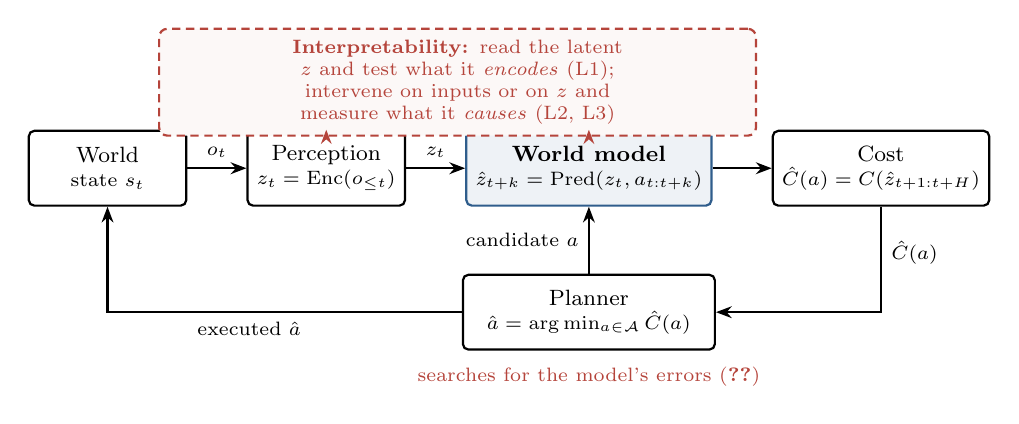
\begin{tikzpicture}[
  box/.style={draw, rounded corners=2pt, minimum height=0.95cm, minimum width=2.0cm, align=center, font=\footnotesize, fill=white, thick},
  wm/.style={box, fill=cblue!8, draw=cblue},
  ar/.style={-{Stealth[length=2mm]}, thick},
  lens/.style={draw=cred, thick, densely dashed, rounded corners=3pt, font=\scriptsize, text=cred, align=center, fill=cred!4, inner sep=4pt},
  node distance=0.5cm and 0.75cm]
\node[box] (world) {World\\[-1pt]\scriptsize state $s_t$};
\node[box, right=of world] (perc) {Perception\\[-1pt]\scriptsize $z_t=\mathrm{Enc}(o_{\le t})$};
\node[wm, right=of perc, minimum width=2.6cm] (wm) {\textbf{World model}\\[-1pt]\scriptsize $\hat z_{t+k}=\mathrm{Pred}(z_t,a_{t:t+k})$};
\node[box, right=of wm] (cost) {Cost\\[-1pt]\scriptsize $\hat C(a)=C(\hat z_{t+1:t+H})$};
\node[box, below=0.85cm of wm, minimum width=3.2cm] (actor) {Planner\\[-1pt]\scriptsize $\hat a=\arg\min_{a\in\mathcal A}\hat C(a)$};
\draw[ar] (world) -- node[above, font=\scriptsize]{$o_t$} (perc);
\draw[ar] (perc) -- node[above, font=\scriptsize]{$z_t$} (wm);
\draw[ar] (wm) -- (cost);
\draw[ar] (cost) |- node[pos=0.22, right, font=\scriptsize]{$\hat C(a)$} (actor);
\draw[ar] (actor.north) -- node[left, font=\scriptsize]{candidate $a$} (wm.south);
\draw[ar] (actor.west) -| node[pos=0.3, below, font=\scriptsize]{executed $\hat a$} (world.south);
\node[lens, above=0.4cm of $(perc)!0.5!(wm)$, text width=7.3cm] (L) {\textbf{Interpretability:} read the latent $z$ and test what it \emph{encodes} (L1);\\ intervene on inputs or on $z$ and measure what it \emph{causes} (L2, L3)};
\draw[cred, thick, densely dashed, -{Stealth[length=1.8mm]}] (L.south -| perc) -- (perc.north);
\draw[cred, thick, densely dashed, -{Stealth[length=1.8mm]}] (L.south -| wm) -- (wm.north);
\node[font=\scriptsize, text=cred, align=center, below=0.08cm of actor] {searches for the model's errors (\cref{prop:optimism})};
\end{tikzpicture}
\caption{\textbf{A world-model-based agent}, following~\citep{lecun2022path}. Every executed action results from a search against the world model's predictions, so the agent's behavior inherits the model's beliefs, including its errors. Interpretability inspects the latent state $z$ shared by perception and prediction.}
\label{fig:arch}
\end{figure}

\Cref{fig:arch} shows the generic structure~\citep{lecun2022path}. An encoder maps observations to a latent state $z_t$, a predictor rolls $z_t$ forward under candidate actions, a cost scores the predicted futures, and a planner searches for the action with the lowest predicted cost. Model-predictive control with a learned model, latent imagination in Dreamer~\citep{hafner2023dreamerv3}, planning in the representation space of a joint-embedding model~\citep{assran2025vjepa2} and policy optimization inside a generative simulator~\citep{nvidia2025cosmos} are all instances. Two properties drive our argument. First, \textbf{the latent is the agent's belief about the world}: if a physical variable is absent from $z$ the agent cannot act on it, and if $z$ encodes it through a correlate, the agent acts on the correlate. Second, \textbf{the planner is an optimizer}: executed actions are not samples from the data distribution but minimizers of a function computed by the model.

%=====================================================================
\section{Why behavioral evaluation is not enough}\label{sec:argument}
%=====================================================================
\subsection{Accuracy does not identify mechanism}\label{sec:formal}
Let the physical state be $s=(q,\lambda)$, with dynamic state $q$ and physical parameters $\lambda$ (mass, friction, gravity), and let $c$ be a \emph{nuisance}: a variable that affects appearance but not dynamics (color, texture, lighting). Observations are $o=\rho(s,c)$ for an injective renderer $\rho$, and future states are $q_{t+1:t+H}=\Phi(q_t,\lambda)$.

\begin{definition}
For a map $\psi$ from nuisances to parameters, the \emph{causal} world model predicts $f_{\mathrm c}(o)=\Phi(q,\lambda)$, and the \emph{$\psi$-shortcut} model predicts $f_{\mathrm s}(o)=\Phi(q,\psi(c))$.
\end{definition}

\begin{proposition}[Behavioral indistinguishability]\label{prop:indist}
If $\lambda=\psi(c)$ almost surely under the data distribution $P$, then $f_{\mathrm c}=f_{\mathrm s}$ $P$-a.s. Hence, for every loss and every test-set size, their empirical risks on i.i.d.\ samples from $P$ are equal with probability one.
\end{proposition}

\begin{proposition}[Separation by intervention]\label{prop:sep}
Let $\mathrm{do}(c\!\leftarrow\!c')$ change the nuisance with $s$ fixed, and let $\Delta(f)=\E\|f(\rho(s,c'))-f(\rho(s,c))\|$. Then $\Delta(f_{\mathrm c})=0$, while $\Delta(f_{\mathrm s})=\E\|\Phi(q,\psi(c'))-\Phi(q,\psi(c))\|>0$ whenever $\Phi$ depends on $\lambda$ on a set of positive probability on which $\psi(c')\neq\psi(c)$.
\end{proposition}

Both proofs are one line (\cref{app:proofs}), and their simplicity is the point. No amount of in-distribution testing can rule out a shortcut; this is a sharp instance of underspecification~\citep{damour2022underspecification} and shortcut learning~\citep{geirhos2020shortcut}. Interventions can rule it out, but designing one requires knowing \emph{which} variable to intervene on. In real scenes the candidate nuisances (lighting, weather, texture, sensor artifacts, co-occurring objects) are combinatorially many, and \cref{prop:indist} says the data gives no hint which ones matter. Reading the model's internal variables changes the search: locate the representation of $\lambda$, ask what it is aligned with, and intervene on that. This is the sense in which black-box access is insufficient for rigorous audits~\citep{casper2024blackbox}. With an imperfect correlation, $\lambda=\psi(c)+\varepsilon$, the risks differ only by terms of order $\varepsilon$, while reading $c$ from pixels may be far easier than inferring $\lambda$ from motion, so training can strictly \emph{prefer} the shortcut. \Cref{sec:exp-val} shows exactly this.

\subsection{Planning turns model error into an adversary}\label{sec:planning}
The next argument is specific to agents that act by optimizing against a world model. Let $C(a)$ be the true cost of action $a$, let $\hat C(a)=C(a)+e(a)$ be the predicted cost, and let the planner execute $\hat a=\arg\min_{a\in\mathcal A}\hat C(a)$ over $N=|\mathcal A|$ candidates.

\begin{proposition}[Planning is optimistic]\label{prop:optimism}
If the model is unbiased at every action, $\E[e(a)]=0$, then $\E[\hat C(\hat a)]\le\min_{a}C(a)\le\E[C(\hat a)]$. If the true costs are equal and the errors are i.i.d.\ with standard deviation $\sigma$, the expected optimism is $\E[C(\hat a)-\hat C(\hat a)]=\sigma\,\E[\max_{a}\xi_a]$, where $\xi_a=-e(a)/\sigma$. This is non-decreasing in $N$, and for Gaussian errors it grows as $\sigma\sqrt{2\log N}$.
\end{proposition}

This is the optimizer's curse of decision analysis~\citep{smith2006optimizer}, a form of Goodhart's law~\citep{goodhart}, and it is known in model-based RL as model exploitation~\citep{janner2019mbpo}. Its consequence for evaluation is what matters here. Held-out loss measures $e$ on actions drawn from the data, but the agent executes the actions on which $e$ is most negative. A stronger planner compares more options and concentrates its choices more sharply on the model's errors, so \emph{improving the planner without improving the model makes realized outcomes worse relative to predictions}. A shortcut model is not even unbiased: it is systematically wrong wherever nuisance and physics disagree, and an agent that chooses where to drive, what to grasp or when to move can steer into those situations. Interpretability addresses this at the right level. It asks whether the variables on which the chosen action depends are the right variables, which does not depend on which actions the planner happens to select.

\subsection{Physical failures are irreversible and rare}
To show with confidence $1-\alpha$ that a per-trial failure probability is below $p$ from failure-free trials alone requires $n\ge\ln(1/\alpha)/p\approx3/p$ trials at 95\% confidence. For automated driving this means hundreds of millions of miles~\citep{kalra2016driving}, and open-world long tails make coverage arguments fragile~\citep{koopman2016challenges}. Combined with \cref{prop:optimism}, the rare situations that matter are the ones the planner is most likely to misjudge. The investigation of the 2018 Tempe collision found that the system detected the pedestrian but repeatedly changed its classification, and did not carry trajectory predictions across those changes~\citep{ntsb2019uber}: the failure lived in an internal representation. Mechanistic evidence scales differently from behavioral evidence. One verified statement about a mechanism covers every situation in which that mechanism is used, including those never observed. Safety cases under functional-safety and AI standards~\citep{iso26262,iso8800,ul4600}, and documentation duties under the EU AI Act~\citep{euaiact2024}, are naturally discharged by evidence of this kind.

%=====================================================================
\section{What interpretability must deliver}\label{sec:levels}
%=====================================================================
\begin{table}[t]
\centering\small
\caption{\textbf{Levels of evidence} about a physical world model. Each level is strictly more informative than the one above it. A certification argument should state the level it relies on.}\label{tab:levels}
\begin{tabular}{@{}L{0.55cm}L{3.0cm}L{3.9cm}L{4.3cm}@{}}
\toprule
& Evidence & Establishes & Fails when \\ \midrule
L0 & held-out behavior & average accuracy on the data distribution & shortcuts (\cref{prop:indist}); planner-induced shift (\cref{prop:optimism}) \\
L1 & probes, feature discovery & variable is \emph{decodable} from $z$ & decodable but unused~\citep{elazar2021amnesic} \\
L2 & interventions on inputs or $z$ & variable is \emph{used} as hypothesized & wrong hypothesis; linear edits miss nonlinear features \\
L3 & circuits and features & \emph{how} the variable is computed and used & incomplete decomposition \\
\bottomrule
\end{tabular}
\end{table}

``Interpretability'' covers methods of very different evidential strength~\citep{doshivelez2017rigorous}. For physical AI the key distinction is between what a representation \emph{encodes} and what it \emph{causes} (\cref{tab:levels}). A linear probe~\citep{alain2016probes} establishes recoverability, not use~\citep{belinkov2022probing,elazar2021amnesic}; interventions on inputs or internal states~\citep{geiger2021causal,meng2022rome,wang2023ioi} establish use. Three desiderata follow from \cref{sec:argument}. Evidence should be \textbf{grounded}: stated in terms of physical variables with a meaning independent of the model (pose, velocity, mass, friction, contact, identity). It should be \textbf{causal}: L2 or above. And it should be \textbf{decision-relevant}: about the variables on which the planner's chosen actions depend, since those are the ones \cref{prop:optimism} says will be stress-tested. Physical AI has one advantage over language here: ground-truth variables are defined by physics and measurable exactly in simulation.

%=====================================================================
\section{Experiments}\label{sec:exp}
%=====================================================================
We instantiate \cref{prop:indist,prop:sep,prop:optimism} in a setting small enough to measure everything. The goal is to exhibit the mechanisms concretely, not to estimate how prevalent they are in deployed systems.

\begin{figure}[t]
\centering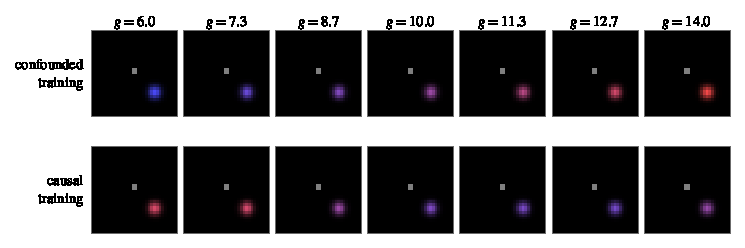
\includegraphics[width=\linewidth]{fig_frames.pdf}
\caption{\textbf{Model inputs} (actual $32{\times}32$ renders). Top: in confounded training data, bob color tracks gravity (blue = low, red = high). Bottom: in causal training data, color is independent of gravity. Within each row, gravity increases from left to right at a fixed angle; the motion that would reveal gravity spans only three frames.}
\label{fig:frames}
\end{figure}

\textbf{Setup.} A damped pendulum, $\ddot\theta=-g\sin\theta-b\dot\theta$, with per-episode $g\sim\mathcal U[6,14]$ and $b\sim\mathcal U[0.05,0.3]$, rendered as $32{\times}32$ RGB frames ($\Delta t=0.08$\,s). The bob's redness $r\in[0,1]$ is a nuisance. With \emph{causal data}, $r$ is independent of the physics; with \emph{confounded data}, $r=(g-6)/8+\mathcal N(0,0.03^2)$ (\cref{fig:frames}). The world model encodes three stacked frames into $z_t\in\mathbb R^{32}$, rolls the latent forward $H=8$ steps (0.64\,s) with a residual MLP, and decodes each predicted frame; it is trained on a foreground-weighted pixel loss (\nEpochs{} epochs, \nTrainWin{} windows, \nSeeds{} seeds per condition). Angles are read from decoded frames with a thresholded centroid (error \readErrMeanMean{} mrad on ground truth). Test sets: \emph{matched}, \emph{decorrelated} (color independent of $g$), \emph{OOD gravity} ($g\in[16,22]$), \emph{OOD damping} ($b\in[0.6,1]$). Results are mean\,$\pm$\,s.d.\ over seeds. Details are in \cref{app:details}.

\subsection{Validation loss prefers the wrong physics}\label{sec:exp-val}
\begin{figure}[t]
\centering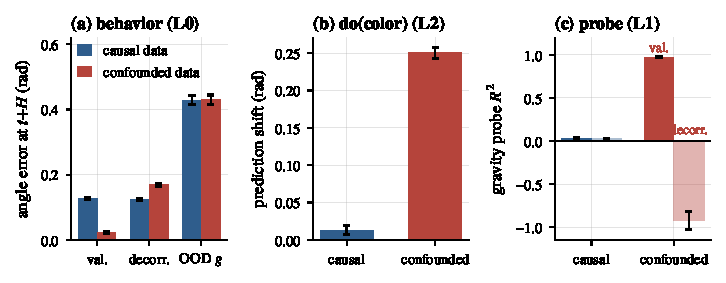
\includegraphics[width=\linewidth]{fig_main.pdf}
\caption{\textbf{Behavior hides the shortcut; interpretability exposes it.} (a) Angle error at the prediction horizon: the confounded-data model is \emph{better} on validation and degrades once color is decorrelated from gravity. (b) Intervening on color with physics held fixed moves only the shortcut model's predictions. (c) Gravity is decodable from the shortcut model's latent on validation data (solid) but not on decorrelated data (hatched). Error bars: s.d.\ over \nSeeds{} seeds.}
\label{fig:main}
\end{figure}

On validation data the confounded-data model is \ratioValClCo$\times$ more accurate (\errCoValMean{} vs.\ \errClValMean{} rad; \cref{fig:main}a), and this ordering holds in \valPicksShortcut{} of \nSeeds{} seeds: model selection by validation loss chooses the shortcut every time. When color is decorrelated from gravity, its error rises \ratioDecVal$\times$ to \errCoDecMean{} rad, while the causal model is unaffected (\errClDecMean{} rad). Behavioral evaluation on the available data does not merely miss the problem; it ranks the two models in the wrong order. Neither model extrapolates to unseen gravity (both errors are above 0.4 rad), which is expected.

Why is the shortcut preferred? Triangulation (\cref{app:triangulation}) gives a precise answer. From three \emph{exact} simulator angles, a finite-difference estimator recovers gravity almost perfectly ($R^2=\idExactMean$). From angles read off $32{\times}32$ pixels it fails ($R^2=\idPixelMean$), because double differencing amplifies milliradian readout error by a factor of order $1/\Delta t^2$. Gravity is barely identifiable from motion at this resolution, and color is the only cheap route to it.

\subsection{Interpretability detects the shortcut before deployment}\label{sec:exp-interp}
\begin{table}[t]
\centering\small
\caption{\textbf{Interpretability evidence}, computed from training-distribution data and synthetic interventions only. Mean\,$\pm$\,s.d.\ over \nSeeds{} seeds.}\label{tab:interp}
\begin{tabular}{@{}llcc@{}}\toprule
& Measurement & Causal data & Confounded data \\ \midrule
\multirow{4}{*}{L1} & probe $R^2$, gravity (val.\ / decorr.) & \rtwoClgravityValMean{} / \rtwoClgravityDecMean & \rtwoCogravityValMean{} / \rtwoCogravityDecMean \\
& probe $R^2$, angular velocity & \rtwoClomegaVal & \rtwoCoomegaVal \\
& cosine(gravity probe, color probe) & n/a$^\ast$ & \cosGRCo \\
& nonlinear probe $R^2$, gravity (MLP / $k$NN) & \idMlpMean{} / \idKnnMean & -- \\ \midrule
\multirow{3}{*}{L2} & do(color): prediction shift at $t{+}H$ (rad) & \intShiftCl & \intShiftCo \\
& do(color): implied gravity shift per unit $r$ & \intGimpCl & \intGimpCo \\
& latent steer: color dir.\ / random dir.\ (rad) & \steerCClMean{} / \steerRClMean & \steerCCoMean{} / \steerRCoMean \\ \bottomrule
\multicolumn{4}{@{}l}{\footnotesize $^\ast$Not meaningful: the causal model's gravity probe has $R^2\approx0$.}
\end{tabular}
\end{table}

\textbf{What the latent encodes (L1).} Both models represent the dynamic state (angular-velocity $R^2\ge$ \rtwoCoomegaValMean). In the shortcut model, gravity is decodable on validation data ($R^2=\rtwoCogravityValMean$), but its probe is nearly parallel to the color probe (cosine \cosGRCoMean) and collapses on decorrelated data ($R^2=\rtwoCogravityDecMean$). Read directly from training data, this says that \emph{the model's gravity variable is a color variable}. The causal model has no gravity variable at all, linear or nonlinear (\cref{tab:interp}), consistent with the identifiability result above.

\textbf{What the latent causes (L2).} Swapping the red and blue channels ($r\to1-r$, physics fixed) moves the shortcut model's prediction by \intShiftCoMean{} rad, \ratioIntCoCl$\times$ the causal model's \intShiftClMean{} rad (\cref{fig:main}b). Fitting $\ddot\theta=-g\sin\theta-b\dot\theta$ to each model's own rollouts recovers the gravity it \emph{behaves as if it believes}. Under the intervention, this shifts by \intGimpCoMean{} per unit redness in the shortcut model, close to the full width (8) of the training range of gravity, and by \intGimpClMean{} in the causal model. This is \cref{prop:sep} observed in trained networks, and graded interventions give a monotone dose-response (\cref{app:triangulation}).

\textbf{Decodable is not the same as used.} Steering $z$ along the probed color direction (changing probed redness by $\pm0.5$) leaves predicted motion essentially unchanged: \steerCCoMean{} rad, no more than a random direction of equal norm (\steerRCoMean{} rad). The dynamics module reads color through a feature that a linear probe does not isolate, reproducing in a world model the gap between decodability and use documented by amnesic probing~\citep{elazar2021amnesic}. A certification argument resting on probes alone would be unsound, which is why \cref{tab:levels} separates L1 from L2.

\subsection{Planning amplifies model error}\label{sec:exp-plan}
\begin{figure}[t]
\centering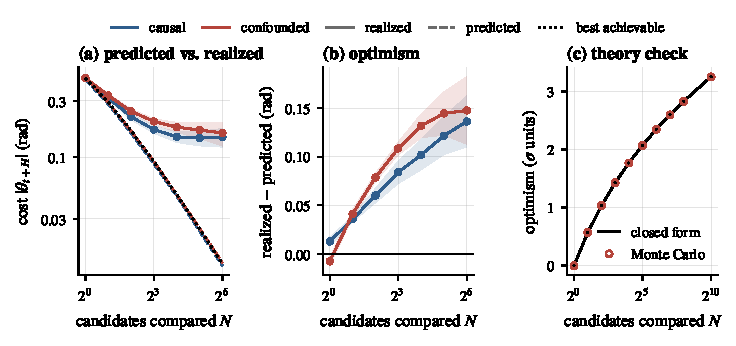
\includegraphics[width=\linewidth]{fig_planner.pdf}
\caption{\textbf{Planning against a world model is optimistic (\cref{prop:optimism}).} (a) A planner picks, among $N$ candidate situations, the one whose \emph{predicted} cost is lowest. Predicted cost (dashed) tracks the best achievable cost (dotted), but realized cost (solid) plateaus. (b) Optimism (realized minus predicted) grows with $N$ for both models, and faster for the shortcut model. (c) Theory check: for unbiased Gaussian errors, Monte Carlo optimism matches the closed form of \cref{prop:optimism}. Bands: s.d.\ over \nSeeds{} seeds.}
\label{fig:planner}
\end{figure}

We test \cref{prop:optimism} with the trained models. A planner faces $N$ candidate situations, drawn from deployment data in which color is independent of physics, and chooses the one whose predicted cost $|\hat\theta_{t+H}|$ (``be at the bottom of the swing at the decision horizon'') is lowest. We record the predicted and realized cost of the chosen situation over 3{,}000 draws per $N$ (\cref{fig:planner}).

The predicted cost falls to \plPredClMean{} rad at $N=\plNmax$, tracking the best achievable cost (\plBestMean{} rad) almost exactly; by its own account, the model is choosing well. The realized cost plateaus at \plRealClMean{} rad for the causal model and \plRealCoMean{} rad for the shortcut model, \plRatio$\times$ worse than predicted. Optimism rises from \plOptOneClMean{} at $N=1$ to \plOptClMean{} rad at $N=\plNmax$ for the causal model, and to \plOptCoMean{} rad for the shortcut model. The shortcut model realizes a higher cost than the causal model for every $N\in\{2,\dots,16\}$ in every seed. For larger $N$ the two models converge, and in one seed the ordering reverses. None of this is visible in held-out loss, which is computed at $N=1$. For unbiased Gaussian errors the closed form is exact: at $N=1024$, Monte Carlo gives \gcMC$\sigma$ against \gcExact$\sigma$ predicted (\cref{fig:planner}c).

\subsection{One can monitor only what the model represents}\label{sec:exp-mon}
Runtime monitors should flag, \emph{before} the agent acts, inputs on which the model is likely wrong. We evaluated four pre-action scores (pixel $k$NN distance; latent Mahalanobis distance~\citep{lee2018mahalanobis}; a gravity-probe range check; and a kinematic-consistency score comparing probed imagined acceleration with observed acceleration) against a lagged baseline, the one-step residual, which needs the next frame. All pre-action scores are near chance under out-of-range gravity (best AUROC \aucClGKnnMean; \cref{app:monitor}), while the lagged residual reaches \aucClGLagMean. The gravity-probe monitor fails for the reason \cref{sec:exp-interp} exposed: the causal model has no gravity variable to read. We take this as support for the thesis rather than a weakness. A monitor built on a model's internal variables is only as good as the model's representation of the variables that matter, so physical world models should be \emph{built} to represent safety-relevant parameters explicitly and \emph{verified} (L1 and L2) to do so before monitors are built on top of them.

%=====================================================================
\section{Related work}
%=====================================================================
\textbf{World models.} Learned world models range from latent dynamics for control~\citep{ha2018world,hafner2023dreamerv3} through joint-embedding predictive architectures~\citep{lecun2022path,assran2023ijepa,assran2025vjepa2} to generative world simulators~\citep{bruce2024genie,nvidia2025cosmos}, and they increasingly underlie robot policies~\citep{brohan2023rt2,kim2024openvla,black2024pi0}. Physics-structured models make some variables explicit by design~\citep{greydanus2019hamiltonian}.
\textbf{Interpretability.} Probing~\citep{alain2016probes,belinkov2022probing} and its limits~\citep{elazar2021amnesic}; causal interventions and causal abstraction~\citep{geiger2021causal,meng2022rome,wang2023ioi}; circuits and dictionary features~\citep{olah2020zoom,elhage2022superposition,bricken2023monosemanticity,templeton2024scaling}; concept vectors~\citep{kim2018tcav}. Emergent world representations have been found in sequence models~\citep{li2023othello,nanda2023emergent,gurnee2023space}, and accurate generative models can hold incoherent world models~\citep{vafa2024evaluating}. Our work brings these tools to physical world models and argues that they are necessary, not optional.
\textbf{Robustness and evaluation.} Underspecification~\citep{damour2022underspecification}, shortcut learning~\citep{geirhos2020shortcut}, goal misgeneralization~\citep{langosco2022goal} and invariant learning~\citep{arjovsky2019irm,scholkopf2021causal} motivate \cref{prop:indist}. Out-of-distribution detection~\citep{hendrycks2017baseline,lee2018mahalanobis,lakshminarayanan2017ensembles} motivates \cref{sec:exp-mon}. The optimizer's curse~\citep{smith2006optimizer} and model exploitation~\citep{janner2019mbpo} motivate \cref{prop:optimism}. Arguments for interpretable models in high-stakes settings~\citep{rudin2019stop,doshivelez2017rigorous,casper2024blackbox} and for the limits of behavioral testing in autonomy~\citep{kalra2016driving,koopman2016challenges} are closest in spirit; we contribute the planning-specific argument and an empirical demonstration in world models.

%=====================================================================
\section{Discussion}
%=====================================================================
\textbf{Objections.} \emph{``More diverse data will fix this.''} Diversity along the right axes helps, but \cref{prop:indist} says the data cannot reveal which axes those are, and \cref{prop:optimism} says the planner will find the ones that were missed; interpretability tells us where to diversify. \emph{``Interpretability does not scale.''} Feature discovery now runs on production-scale models~\citep{templeton2024scaling}, and physical world models have an advantage that language models lack: their ground-truth variables are measurable in simulation. \emph{``Explanations can be unfaithful.''} They can~\citep{adebayo2018sanity,elazar2021amnesic}, and our steering result reproduces this. The remedy is to require causal (L2+) evidence, not to abandon interpretability.

\textbf{A research program.} (1) \emph{Physical-variable audits}: for every safety-relevant variable, report L1 decodability and L2 causal use on simulation suites with known ground truth, alongside benchmark numbers. (2) \emph{Interpretability-guided stress tests}: use feature discovery on world-model latents to \emph{propose} candidate nuisances, and test each with interventions. (3) \emph{Decision-focused analysis}: evaluate on planner-selected states, not only on the data distribution (\cref{prop:optimism}). (4) \emph{Causal methods for latent dynamics}: extend interchange interventions~\citep{geiger2021causal} to recurrent predictors, since linear edits missed the feature the shortcut used. (5) \emph{Representation-aware training}: objectives that make physical parameters identifiable in $z$~\citep{scholkopf2021causal,bengio2013representation}, mindful that this requires inductive bias~\citep{locatello2019challenging}.

\textbf{Limitations.} Our experiments use one low-dimensional system, one designed confound and a small world model. They demonstrate mechanisms, not their prevalence; validating on large world models with naturally occurring confounds is the most important next step. Our confound is nearly deterministic, and weaker confounds will weaken the preference for the shortcut. Our monitors were simple, and our planner selects among sampled situations rather than optimizing continuous action sequences. Regulatory requirements vary by jurisdiction, and we offer no legal interpretation.

\section{Conclusion}
An agent that acts by consulting a world model is only as trustworthy as that model's beliefs about how the world works, and those beliefs cannot be read off its accuracy. A world model can be more accurate on everything that was tested and still wrong about the world; a planner that optimizes against it will find where it is wrong; and in the physical world those situations are rare, consequential and irreversible. Verifying a world model's beliefs requires examining the variables it represents and testing what they cause. That is why physical AI must be interpretable, and why the interpretability it needs must be causal.

\section*{Broader impact}
This work argues for stronger verification of physical AI before deployment, which we expect to reduce harm from autonomous systems. A risk is that interpretability evidence is over-trusted: probes can mislead (\cref{sec:exp-interp}), and an audit at one level should not be presented as evidence at a higher one. Our experiments involve only simulation.

{\small
\bibliographystyle{plainnat}
\bibliography{refs}}

\newpage
\appendix
\section{Proofs}\label{app:proofs}
\textbf{\Cref{prop:indist}.} On the support of $P$, $\psi(c)=\lambda$, so $\Phi(q,\psi(c))=\Phi(q,\lambda)$ pointwise, and empirical risks are sums of identical terms.
\textbf{\Cref{prop:sep}.} $f_{\mathrm c}$ does not depend on $c$; for $f_{\mathrm s}$, substitute the definition.
\textbf{\Cref{prop:optimism}.} The minimum is concave, so by Jensen's inequality $\E[\min_a\hat C(a)]\le\min_a\E[\hat C(a)]=\min_aC(a)$, and the left side equals $\E[\hat C(\hat a)]$. Pointwise $C(\hat a)\ge\min_aC(a)$. With equal true costs, $C(\hat a)-\hat C(\hat a)=-e(\hat a)=\max_a(-e(a))$. Adding candidates cannot decrease a maximum, and $\E[\max_{a\le N}\xi_a]\sim\sqrt{2\log N}$ for i.i.d.\ standard Gaussians.

\section{Implementation details}\label{app:details}
\textbf{Simulation.} Semi-implicit Euler with 10 substeps per frame; $\theta_0\sim\mathcal U[-1.4,1.4]$, $\dot\theta_0\sim\mathcal U[-2,2]$. The bob is a Gaussian blob (s.d.\ 1.6\,px) at radius 11\,px, with RGB color $(0.3+0.7r,\,0.3,\,0.3+0.7(1-r))$. Windows of 3 input and 8 target frames, stride 3.
\textbf{Model.} Encoder: three stride-2 $4{\times}4$ convolutions (32/64/64 channels, GELU), then an MLP to $\mathbb R^{32}$. Predictor: residual MLP (two hidden layers of 256). Decoder: MLP then three transposed convolutions with linear output. Loss weight $1+30\max_c y$ (without it, training collapses to an empty frame). AdamW, learning rate $10^{-3}$, one-cycle schedule, weight decay $10^{-4}$, batch 128, gradient clipping at norm 1. About 4 minutes per model on 2 CPU cores.
\textbf{Analyses.} Probes: ridge regression with cross-validated $\alpha\in[10^{-3},10^3]$, fit on training windows. Implied gravity: least-squares fit of the pendulum equation to finite differences of predicted angles. Latent steering: $z\leftarrow z+\delta\,w/\|w\|^2$ with $w$ the redness-probe weights and $\delta=\pm0.5$; the control uses a Gaussian direction of equal norm. Planner: 3{,}000 random candidate sets per $N$, drawn from 300 decorrelated episodes per seed.

\section{Triangulation}\label{app:triangulation}
Each headline claim was re-derived with an independent method. Physics oracles are simulations and cannot be influenced by any training choice.
\begin{table}[h]\centering\small
\begin{tabular}{@{}llc@{}}\toprule
Check & Measurement & Value \\ \midrule
Argmax-pixel readout (independent) & causal / confounded, validation (rad) & \triArgClValMean{} / \triArgCoValMean \\
& confounded, decorrelated (rad) & \triArgCoDecMean \\
Physics oracles, decorrelated (rad) & true $g$ / mean $g$ / $g$ from color & \oraTrueGMean{} / \oraMeanGMean{} / \oraColGMean \\
& causal model / shortcut model & \oraModelClMean{} / \oraModelCoMean \\
Gravity identifiability ($R^2$) & exact angles / pixel readout & \idExactMean{} / \idPixelMean \\
Dose-response, shortcut (rad) & $\Delta r=0.05,0.1,0.2,0.3$ & \doseACoMean, \doseBCoMean, \doseCCoMean, \doseDCoMean \\
Dose-response, causal (rad) & $\Delta r=0.3$ & \doseDClMean \\ \bottomrule
\end{tabular}
\caption{Triangulation, means over \nSeeds{} seeds. Each model's error matches the physics oracle that corresponds to the hypothesis its internals suggest it holds: mean gravity for the causal model, gravity read from color for the shortcut model.}
\end{table}

\section{Additional results}\label{app:monitor}
\begin{figure}[h]
\centering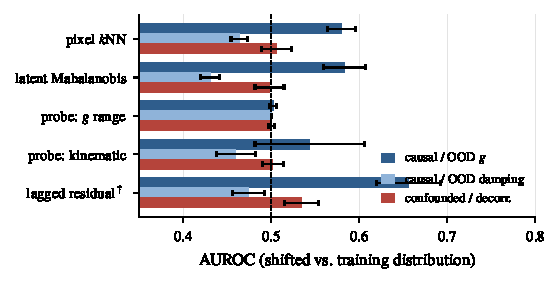
\includegraphics[width=0.62\linewidth]{fig_monitor.pdf}
\caption{Runtime-monitor AUROC (shifted vs.\ training distribution). All scores except the lagged residual ($\dagger$) are available before acting. Dashed line: chance.}
\end{figure}
\begin{table}[h]\centering\small
\begin{tabular}{@{}lcc@{}}\toprule
Angle error at $t{+}H$ (rad) & Causal data & Confounded data \\ \midrule
Validation & \errClVal & \errCoVal \\
Color decorrelated & \errClDec & \errCoDec \\
OOD gravity & \errClOodG & \errCoOodG \\
OOD damping & \errClOodD & \errCoOodD \\ \bottomrule
\end{tabular}
\caption{Behavioral evaluation, mean\,$\pm$\,s.d.\ over \nSeeds{} seeds.}
\end{table}

\section{Reproducibility}\label{app:repro}
All code, per-seed results, checkpoints and the scripts that generate every number and figure are released. No number in the paper is typed by hand: each is a macro generated from stored results. Every empirical claim is an executable check that must hold in \emph{every} seed. A from-scratch retraining reproduces the stored metrics exactly (maximum difference 0). The suite found and corrected an unseeded weight initialization and an overstated readout-accuracy claim during development. A full earlier run with unseeded initialization independently reproduces every headline ratio. Everything runs on two CPU cores in about an hour.

\section{NeurIPS paper checklist}
\begin{enumerate}[leftmargin=1.2em]
\item \textbf{Claims.} [Yes] The abstract and introduction state the scope: a position supported by propositions and controlled toy experiments, with limitations in the Discussion.
\item \textbf{Limitations.} [Yes] Discussion, ``Limitations''.
\item \textbf{Theory, assumptions and proofs.} [Yes] Assumptions are stated in each proposition; proofs are in \cref{app:proofs}.
\item \textbf{Experimental result reproducibility.} [Yes] \cref{app:details,app:repro}; seeds, data streams and versions are pinned.
\item \textbf{Open access to data and code.} [Yes] Released with the paper; the data is generated by the included simulator.
\item \textbf{Experimental setting and details.} [Yes] \cref{sec:exp}, \cref{app:details}.
\item \textbf{Statistical significance.} [Yes] Mean\,$\pm$\,s.d.\ over \nSeeds{} seeds; episode-level bootstrap 95\% CIs (\cref{app:triangulation}); claims must hold in every seed.
\item \textbf{Compute resources.} [Yes] Two CPU cores; about 4 minutes per model; about one hour for the full pipeline.
\item \textbf{Code of ethics.} [Yes] The work conforms to the NeurIPS Code of Ethics.
\item \textbf{Broader impacts.} [Yes] See ``Broader impact''.
\item \textbf{Safeguards.} [N/A] No high-risk models or data are released.
\item \textbf{Licenses for existing assets.} [Yes] Only standard open-source libraries are used; the code is released under Apache-2.0.
\item \textbf{New assets.} [Yes] Code and results are documented in the repository README.
\item \textbf{Crowdsourcing and human subjects.} [N/A]
\item \textbf{IRB approvals.} [N/A]
\item \textbf{Declaration of LLM usage.} An LLM assistant was used for coding, writing and editing; the author is responsible for all content.
\end{enumerate}
\end{document}
